\newpage
\section{Experiment Instructions}
\subsection{CDA} \label{app_instruction_cda}

Welcome, and thank you for participating!

From now until the end of the experiment, please do not communicate with
other participants. Please turn off your cell phones and stay focused on
the task. If you have any questions, please raise your hand or let the
experimenters know; they will answer your questions.

Please pay careful attention to the instructions, as real money is at
stake. During the experiment, you will earn Experimental Currency Units
(ECUs). At the end of the experiment, we will convert your earnings into
US Dollars (USD) at one dollar for every 1000 ECUs. You are guaranteed a
show-up fee of USD 6 but can earn considerably more.

\subsubsection*{Basic Idea}\label{basic-idea_cda}

In this experiment, you and seven other participants will be traders in
a simple automated financial market. Using the information displayed on
your screen, you will make trades to earn as many ECUs as possible. As
explained below, your earnings will depend on the trade offers you and
the other traders make in your group. There will be 22 trading periods,
each lasting 2 minutes.

The two first rounds are practice rounds (they don't count for your actual payment).

Your final earnings for the session will be the sum of your show-up fee
and the cumulative profits from all trading periods, converted into US
Dollars.

\subsubsection*{Buy Orders and Sell Orders (Treat
CDA)}\label{buy-orders-and-sell-orders-treat-cda}

All traders can submit or update \emph{buy} and/or \emph{sell orders}.
Each order consists of \ul{two} elements or pieces of information:

\begin{itemize}
\item
  The \emph{\textbf{total quantity}} stating the number of shares that
  the agent wants to trade.
\item
  The \emph{\textbf{limit price}} of the order. In \ul{buy orders}, the
  limit price indicates the maximum price the trader is willing to pay
  per share. In \ul{sell orders}, the limit price indicates the minimum
  price the trader is willing to accept for each share.
\end{itemize}

\paragraph*{Example}\label{example_cda}

The blue line and blue square in Figure \ref{fig:instuctions_cda_input1} show that the trader submitted
a buy order for a total of 200 shares at a limit price of 13 ECUs. If
someone is willing to sell for 13 ECUs or less, the former trader's buy
order will be filled. If that counterpart wants to trade less than 200
shares, then the order will be filled only partially.

Figure 1 also shows (in red) that the trader submitted a sell order for
100 shares. The limit price of this order is 15 ECUs. That is, if
someone is willing to buy at 15 ECUs or a higher price, the sell order
will be filled. If said counterpart wants to trade less than 100 shares,
then the order will be filled only partially.

\begin{figure}[H]
    \centering
    \caption{CDA Your Input}
    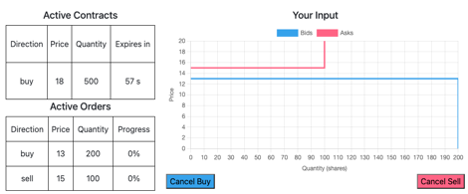
\includegraphics[width=.8\linewidth]{figures/instructions_cda1.png}
    \label{fig:instuctions_cda_input1}
\end{figure}

\paragraph*{Submitting orders in the graphical interface (Treat CDA) }\label{submitting-orders-in-the-graphical-interface-treat-cda}

To set a \ul{sell} order, you drag the red square anywhere inside the
``your input'' grid to set the limit price and the total quantity
(volume). You submit your order by clicking on the ``Send Sell'' red
button, as is shown in Figure \ref{fig:instuctions_cda_input2}.

Similarly, to set a \ul{buy} order, you can drag the blue square
anywhere inside the grid to set the limit price and the total quantity
(volume). Then you can submit your order by clicking on the ``Send Buy''
button.

In case your order is not completely executed, your order will remain
active with the remaining quantity. For example, if your order is for
buying 200 shares and you only obtain 150 shares when trading with
another participant. Then, your order remains active, but now only for
50 shares.

You can submit a new buy (sell) order, or cancel it, at any time.
However, if you have an active order, you first need to cancel it by
pressing the ``cancel buy'' (``cancel sell'') button. Then you can
submit a new order.

\begin{figure}[H]
    \centering
    \caption{CDA Your Input}
    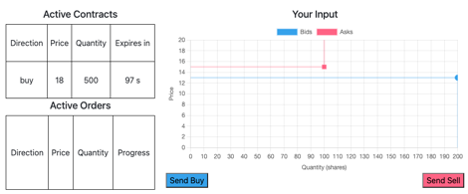
\includegraphics[width=.8\linewidth]{figures/instructions_cda2.png}
    \label{fig:instuctions_cda_input2}
\end{figure}

\subsubsection*{Contracts}\label{contracts_cda}

Why do you want to trade? What is a share worth to you? The answer to
both questions is that the computer will give you a contract that
enables you to profit from trading. You will receive your contract near
the beginning of the trading period, and it will appear in the ``Active
Contracts'' table on the left of the screen, as shown in Figure \ref{fig:instuctions_cda_input1}.

For example, your contract might read \textbf{``Buy 500 shares at a
price of 18 ECUs in 97 seconds.}'' This means that 97 seconds from now,
the computer will buy up to 500 shares from your inventory at a price of
18. To take advantage of this opportunity, you need to buy some shares
to build up your inventory. Your profit on each share (up to the 500th
share) is the contract price (here 18) minus the price you paid when you
bought that share. Of course, for this contract it would not be
worthwhile to buy shares at a higher price than 18 or to buy more than
500 shares.

Similarly, a contract that says \textbf{``Sell 150 shares at a price of
13 ECUs in 80 seconds"} means that, in 80 seconds, the computer will
sell you up to 150 shares at the price of 13 ECUs per share. Here you
make a profit by selling up to 150 shares at prices above 13 ECUs per
share. For this contract, it would not be worthwhile to sell shares at a
lower price than 13 or to sell more than 150 shares.

Keep in mind that you can buy more shares than you have cash for and
thus have a negative cash balance, or sell more shares than you own and
thus have a negative inventory (this is called shorting). If you have a
BUY contract for 400 shares, your inventory should be between zero and
your contract quantity, 400 shares. If you have a SELL contract for 500
shares, your inventory should be between -500 (minus 500) shares and
zero.

\subsubsection*{How the market works (Treat
CDA)}\label{how-the-market-works-treat-cda}

The market price at which you can buy or sell shares depends on other
traders\textquotesingle{} buy and sell orders. Consider the example
illustrated in Figure \ref{fig:instructions_cda_market}. All traders, except Trader 1, have active buy or sell orders. In particular, the four sellers want to sell at prices of 15 or more, respectively (see red steps). These four sellers conform to the market supply (the sum of their four sell orders) shown in red. The four buyers want to buy at prices of 13, 12 and 11 or less,
respectively (see blue steps). These three buyers conform to the market
demand (the sum of their three buy orders) shown in blue.

The green dots indicate the most recent trades. The latest trade is
represented by the largest dot.

As you can see, the demand and supply do not cross each other inside the
box but along the y-axis. That is there cannot be trade at that point.

Let us see what happens when Trader 1 decides to submit a buy order.
There are two cases.

\begin{itemize}
\item
  First, if her buy order has a price below the lowest sell order price
  (say 15), then Trader 1 will only add to the demand, and no
  transaction will occur.
\item
  Second, if Trader 1's buy order comes at a price above the lowest
  selling price (say 13), then she will transact immediately with the
  seller(s) with the lowest price. Suppose the seller with the lowest
  price does not offer enough volume (quantity) to fill Trader's 1
  order. In that case, the buy order of Trader 1 will be filled only
  partially or the remaining quantity will be purchased from the second
  lowest selling price, and so on.
\end{itemize}

\begin{figure}[H]
    \centering
    \caption{CDA Market}
    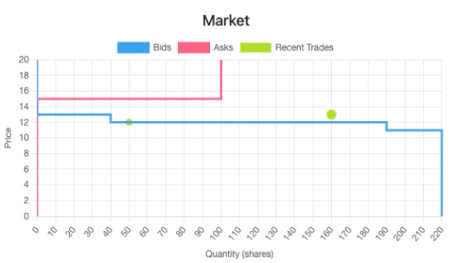
\includegraphics[width=.8\linewidth]{figures/instructions_cda3.png}
    \label{fig:instructions_cda_market}
\end{figure}

\subsubsection*{Your Earnings}\label{your-earnings_cda}

You make a profit by selling shares at higher prices than you bought
them.

However, notice that you do not need to buy a share in order to sell it.
Even if you have zero inventory you can still sell shares (making your
inventory negative). Similarly, even if you have no cash, you can still
buy shares (making your cash balance negative).

Also, notice that you can buy and sell from and to either the computer
and other participant traders, or both. Your profits from transactions
with other participants will appear immediately in your cash account,
whereas your profits from contracts with the computer will be added to
the cash account when the contract expires (aka contract deadline).

\textbf{Examples:} You lose money when you buy at a higher price than
you sold, or sell at a lower price than you bought. For example, suppose
you pay 23 ECUs for one share that you sell to the computer at a contract price of 17 ECUs. Then your profit is 17 - 23 = - 6 ECUs. That is, you incurred a loss of 6 ECUs on that share. If, instead, you bought that share at price of 14 ECUs before the deadline, you would get a profit of 17 - 14 = 3 ECUs on that share.

\textbf{Projected Profits}

The middle bottom box shows your \emph{projected profits} which indicate
your period profits if the active contract (if any) expires immediately
and the period ends right away. This provides a summary of your current
state.

\textbf{Session Dollar Earnings:} After the last trading round, the
computer will add up all your period earnings to determine your actual
compensation. These earnings will be converted into US dollars at one
dollar for every 1000 ECUs.

\begin{figure}[H]
    \centering
    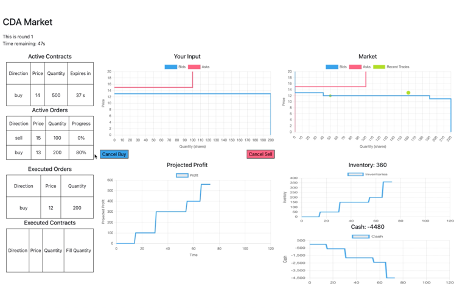
\includegraphics[width=.8\linewidth]{figures/instructions_cda4.png}
    \caption{CDA UI}
    \label{fig:instuctions_cda_all}
\end{figure}


\subsection{FLOW} \label{app_instruction_flow}
Welcome, and thank you for participating!

From now until the end of the experiment, please do not communicate with
other participants. Please turn off your cell phones and stay focused on
the task. If you have any questions, please raise your hand or let the
experimenters know; they will answer them.

Please pay careful attention to the instructions, as real money is at
stake. During the experiment, you will earn Experimental Currency Units
(ECUs). At the end of the experiment, we will convert your earnings into
US Dollars (USD) at one dollar for every 1000 ECUs. You are guaranteed a
show-up fee of USD 6 but can earn considerably more.

\subsubsection*{Basic Idea}\label{basic-idea_flow}

In this experiment, you and seven other participants will be traders in
a simple automated financial market. Using the information displayed on
your screen, you will make trades to earn as many ECUs as possible. As
explained below, your earnings will depend on the trade offers you and
the other traders make in your group. There will be 20 trading periods,
each lasting 2 minutes.

The first two rounds are practice rounds (they don't count for your actual payment).

Your final earnings for the session will be the sum of your show-up fee
and the cumulative profits from all trading periods, converted into US
Dollars.

\subsubsection*{Buy Orders and Sell Orders (Treat
FLOW)}\label{buy-orders-and-sell-orders-treat-flow}

All traders can submit or update \emph{buy} and/or \emph{sell orders}.
Each order consists of four elements:

\begin{itemize}
\item
  The \emph{\textbf{total quantity}} stating the number of shares that
  the agent wants to trade,
\item
  The \emph{\textbf{maximum rate}} of shares to trade per second.
\item
  The \emph{\textbf{low price}} of the order. In \ul{buy orders}, the
  low price indicates the price under which the order is filled at the
  \emph{maximum rate.} In \ul{sell orders}, the low price indicates the
  price under which the order is not filled\emph{.}
\item
  The \emph{\textbf{high price}} of the order. In \ul{buy orders}, the
  high price indicates the price above which the order is not
  filled\emph{.} In \ul{sell orders}, the high price indicates the price
  above which the order is filled at the \emph{maximum rate.}
\end{itemize}

\paragraph*{Example}\label{example_flow}

The blue line and blue box in Figure \ref{fig:instructions_flow_input} show that the trader submitted a
buy order for a total of 500 shares at the maximum rate of 15 shares per
second at prices between 6 (low price) and 12 (high price). When the
market price is at or below 6 ECUs per share, her order will be filled
at her \emph{maximum rate} (15 shares per second). Her buy order will
not be executed when the market price is at or above 12 ECUs per share.
When the market price is between 6 to 12 ECUs per share, her order will
be filled at a rate between zero and her maximum rate. The higher the
market price, the lower the rate of execution.

Figure \ref{fig:instructions_flow_input} also shows (in red) that the trader submitted a sell order for
50 shares. Her \emph{maximum rate} is 19 shares per second, her
\emph{low price} is 14, and her \emph{high price} is 18. When the market
price is at or above 18 ECUs per share, her order will be filled at her
\emph{maximum rate} of 19 shares per second. Her sell order will not be
executed when the market price is at or below 14 ECUs per share. When
the market price is between 14 to 18 ECUs per share, her order will be
filled at a rate between zero and her maximum rate. The higher the
market price, the higher the rate of execution.

\begin{figure}[H]
    \centering
    \caption{FLOW Your Input}
    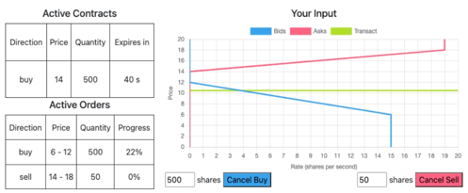
\includegraphics[width=\linewidth]{figures/instruction_flow1.png}
    \label{fig:instructions_flow_input}
\end{figure}

\paragraph*{Submitting orders in the graphical interface (Treat FLOW) }\label{submitting-orders-in-the-graphical-interface-treat-flow}

To set a \ul{sell} order, you move the red dot along the vertical axis
to set the low price, and you drag the red square anywhere inside the
grid to set the high price and maximum rate. You enter the \textbf{total
number of shares} you want to sell in the box next to the ``Send Sell''
red button. When you have finished setting the order, submit your order
by clicking on the ``Send Sell'' button.

Similarly, to set a \ul{buy} order, you move the blue dot along the
vertical axis to set the high price, and you drag the blue square
anywhere inside the grid to set the low price and the maximum rate. You
enter the \textbf{total number of shares} you want to buy in the box
next to the ``Send Buy'' blue button. When you have finished setting the
order, submit your order by clicking on the ``Send Buy'' button.

You can submit a new buy (sell) order, by first canceling your active
buy (sell) orders and then submitting a new buy (sell) order. You do not
need to wait for an order to be fully executed to cancel it.

\subsubsection*{Contracts}\label{contracts_flow}

Why do you want to trade? What is a share worth to you? The answer to
both questions is that the computer will give you a contract that
enables you to profit from trading. You will receive your contract near
the beginning of the trading period, and it will appear in the ``Active
Contracts'' table on the left of the screen, as shown in Figure \ref{fig:instructions_flow_input}.

For example, your contract might read \textbf{``Buy 500 shares at a
price of 14 ECUs in 40 seconds.}'' This means that 40 seconds from now,
the computer will buy up to 500 shares from your inventory at a price of
14. To take advantage of this opportunity, you need to buy some shares
to build up your inventory. Your profit on each share (up to the 500th
share) is the contract price (here 14) minus the price you paid when you
bought that share. Of course, for this contract it would not be
worthwhile to buy shares at a higher price than 14 or to buy more than
500 shares.

Similarly, a contract that says \textbf{``Sell 150 shares at a price of
13 ECUs in 80 seconds"} means that, in 80 seconds, the computer will
sell you up to 150 shares at the price of 13 ECUs per share. Here you
make a profit by selling up to 150 shares at prices above 13 ECUs per
share. For this contract, it would not be worthwhile to sell shares at a
lower price than 13 or to sell more than 150 shares.

Keep in mind that you can buy more shares than you have cash for and
thus have a negative cash balance, or sell more shares than you own and
thus have a negative inventory (this is called shorting). If you have a
BUY contract for 400 shares, your inventory should be between zero and
your contract quantity, 400 shares. If you have a SELL contract for 500
shares, your inventory should be between -500 (minus 500) shares and
zero.

\subsubsection*{How the market works (Treat
FLOW)}\label{how-the-market-works-treat-flow}

The market price and the rate at which you can buy or sell shares
depends on the buy and sell orders of all traders, as illustrated in the
top chart of Figure \ref{fig:instructions_flow_market}. Here, one trader submitted the buy order and sell order shown in Figure \ref{fig:instructions_flow_input}. Together with the buy and sell orders submitted by the other 7 traders, they resulted in the market demand (sum of buy
orders) shown in blue and market supply (summed sell orders) shown in
red. The supply and demand intersect at a price of 10.48 and a Rate of
3.8. Therefore the trader from Figure \ref{fig:instructions_flow_input} is buying at a price of 10.48 ECU to some other trader(s) at a rate of 3.8 shares per second (where the price crosses the agents' demand curve). Thus, her cash position is decreasing at a rate of 10.48 x 3.8 = 19.82 ECU per second while her
inventory is increasing at a rate of 3.8 shares per second. This will continue until she buys her total quantity of 500 shares, or until the other traders change their supply or demand, e.g., when they reach their requested total quantity or when they place a new order.

\begin{figure}[H]
    \centering
    \caption{FLOW Market}
    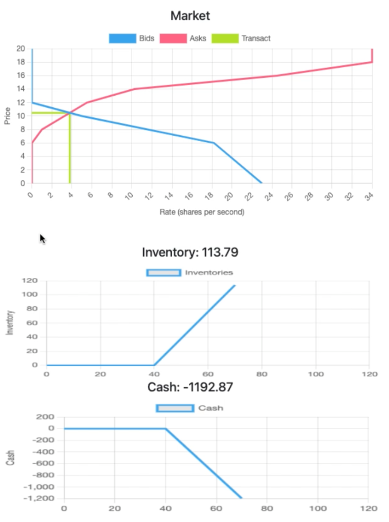
\includegraphics[width=.6\linewidth]{figures/instruction_flow2.png}
    \label{fig:instructions_flow_market}
\end{figure}

\subsubsection*{Your Earnings}\label{your-earnings_flow}

You make a profit by selling shares at higher prices than you bought
them.

However, notice that you do not need to buy a share in order to sell it.
Even if you have zero inventory you can still sell shares (making your
inventory negative). Similarly, even if you have no cash, you can still
buy shares (making your cash balance negative).

Also, notice that you can buy and sell from and to either the computer
and other participant traders, or both. Your profits from transactions
with other participants will appear immediately in your cash account,
whereas your profits from contracts with the computer will be added to
the cash account when the contract expires (aka contract deadline).

\textbf{Examples:} You lose money when you buy at a higher price than
you sold, or sell at a lower price than you bought. For example, suppose
you pay 23 ECUs for one share that you sell to the computer at a
contract price of 17 ECUs. Then your profit is 17 - 23 = - 6 ECUs. That
is, you incurred in a loss of 6 ECU on that share. If, instead, you
bought that share at price of 14 ECUs before the deadline, you would get
a profit of 17 - 14 = 3 ECUs on that share.

\textbf{Projected Profits}

The middle bottom box shows your \emph{projected profits} which indicate
your period profits if the active contract (if any) expires immediately
and the period ends right away. This provides a summary of your current
state.

\textbf{Session Earnings:} After the last trading period, the computer
will add up all your period earnings to determine your actual
compensation. These earnings will be converted into US Dollars at a rate
of one US Dollar for every 1000 ECUs.

\begin{figure}[!htbp]
    \centering
    \caption{FLOW UI}
    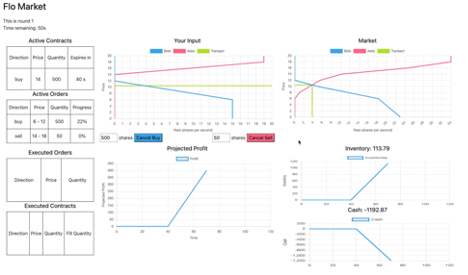
\includegraphics[width=\linewidth]{figures/instruction_flow3.png}
    \label{fig:instructions_flow_all}
\end{figure}

